% Created 2018-03-16 Fri 17:11
\documentclass{article}
\usepackage[mathletters]{ucs}
\usepackage[utf8x]{inputenc}
\usepackage[T1]{fontenc}
\usepackage{fixltx2e}
\usepackage{graphicx}
\usepackage{longtable}
\usepackage{float}
\usepackage{wrapfig}
\usepackage{rotating}
\usepackage[normalem]{ulem}
\usepackage{amsmath}
\usepackage{textcomp}
\usepackage{marvosym}
\usepackage{wasysym}
\usepackage{amssymb}
\usepackage{hyperref}
\tolerance=1000
\usepackage[margin=1.0in]{geometry}
\date{\today}
\title{Notebook2}
\hypersetup{
  pdfkeywords={},
  pdfsubject={},
  pdfcreator={Emacs 25.3.1 (Org mode 8.2.10)}}
\begin{document}

\maketitle
\tableofcontents

\section{Implementing Low and High Pass Image Filters}
\label{sec-1}
\begin{itemize}
\item Instead of doing my initial spiel about high and low pass filters, I
will instead discuss the relevant information after I implement
\texttt{lowPass} and \texttt{highPass} and before Ι talk about the results found.
\end{itemize}
\begin{enumerate}
\item Setup
\label{sec-1-1}
\begin{itemize}
\item Since we need to read images, Ι bring some functions to convert
images into a proper REPA Array (REPA are just very quick and parallel
arrays Ι use), and make two additional functions
\begin{verbatim}
repaRGBToGrey :: (Integral b, Source r b) ⇒ Array r DIM3 b → Array D DIM2 b
repaRGBToGrey arr = R.traverse arr (\_ → ix2 i j) average
  where (Z :. i :. j :. _)    = R.extent arr
        getAll3 (Z :. i :. j) = (\k -> Z :. i :. j :. k) <$> [0..2]
        average f sh          = round $ sum (fromIntegral ∘ f <$> getAll3 sh) / 3

saveRepaGrey :: (RealFrac a, Source r a) ⇒ FilePath → Array r DIM2 a → IO ()
saveRepaGrey loc = savePngImage loc ∘ ImageY8 ∘ repaToGreyImage
\end{verbatim}
\begin{itemize}
\item here \texttt{repaRGBToGrey} just turns a 3d array into a grey one by
adding all values over the third dimension then dividing by 3,
giving us a new array
\item saveRepaGrey is just a useful function that converts our 2D array
into an Image which I then save, so I don't have to call all the
transformations all the time.
\end{itemize}
\end{itemize}
\item Implementations
\label{sec-1-2}
\begin{itemize}
\item I ended up trying two different discrete cosine transformers, as
when I test dct composed with idct Ι did not get the same vector
back. Ι eventually managed to get the first one working, by noticing
that the value returned from \texttt{(dct · idct) vec =} $\frac{vec}{\text{length(vec)} * 2}$
\item with that said, Ι will now talk about the successful attempt.
\item So I notice an import in the "statistics" package has a discrete
cosine transformer and its inverse, so Ι decided to use that
\begin{verbatim}
repaVecComp :: Shape sh ⇒ (V.Vector e1 → V.Vector e2) → Array V sh e1 → Array V sh e2
repaVecComp f arr = fromVector (R.extent arr) (f (toVector arr))

repaDctImage :: Shape sh ⇒ Array V sh Double → Array V sh Double
repaDctImage = repaVecComp (dct . fmap (+ (-128)))

-- For some reason repaDct ∘ repaIDct doesn't give me the identity
-- Ι have to divide it by twice the length
repaIDctImage :: Shape sh ⇒ Array V sh Double → Array V sh Double
repaIDctImage = repaVecComp (normalize . idct)
   where normalize v = (+ 128) . (/ (fromIntegral (length v) * 2)) <$> v
\end{verbatim}
\begin{itemize}
\item to get the dct and idct function to work, Ι had to convert our array
to a vector (this is O(1) as it just unpacks!), so I make a
generic function called repaVeccomp that does some computation in
the vector plane before giving me back the array. With this
defined I just pass \texttt{dct} for \texttt{repaDct} and \\ \texttt{((\textbackslash{}v → fmap (/
    (fromIntegral (length v) * 2)) v) ∘ idct)} for idct (offset
described above!).

\item I include a -128 offset as we want the image to be centered around
0 before we do our high/low pass filter

\item Ι also have repaDct, repaIDct variants which don't have the offset.

\item Also not shown is repaDctImageP and repaIDctImageP which have the
offsets and also compute the vectors in parallel.
\end{itemize}

\item Ι can now check if these functions work as expected by the following
function
\begin{verbatim}
testsame :: Bool
testsame = (round <$> toList (id vec)) == [1,2,3,4]
  where id  = repaIDct ∘ repaDct
        vec = fromVector (ix2 2 2) (V.fromList [1,2,3,4])
\end{verbatim}
\begin{itemize}
\item This function returns true, and is really just confirms that
\texttt{repaIDct} ∘ \texttt{repaDct} is really the identity.
\end{itemize}

\item Now we are ready to implement the pass Filters.
\begin{verbatim}
-- type signature slightly simplied for pdf
genPass :: (Int → Int → Bool) → Int → Array r DIM2 b → Array D DIM2 b
genPass (<>) n arr = R.traverse arr id shrink
  where shrink f sh@(Z :. i :. j)
          | i <> n ∧ j <> n = f sh
          | otherwise       = 0


lowPass :: (Source r b, Num b) ⇒ Int → Array r DIM2 b → Array D DIM2 b
lowPass = genPass (≤)

highPass :: (Source r b, Num b) ⇒ Int → Array r DIM2 b → Array D DIM2 b
highPass = genPass (≥)
\end{verbatim}
\begin{itemize}
\item What genPass does is zero out a region if the predicate isn't
true, so for the lowPass, only the top left is kept in tact since
$i ≥ n ∧ j ≥ n$ must be true. and for highPass only the bottom
right is kept in tact as $i ≤ n ∧ j ≤ n$ must be true else the
region is 0.

\begin{itemize}
\item One mistake that Ι did earlier was using ∨ instead of ∧ which
changed some results, which I'll compare and contrast some of it,
since notebook1 gives us the intuition to do so.
\end{itemize}

\item Now let's discuss what frequencies these high and low pass filters
filter out. So the low pass filter lets the low frequencies
through and zeros out the high frequencies, and if you were to compare
our operations to the diagram in notebook1 you'll notice that this
corresponds to the region where there is a very slow shift of
values. Where as the high pass removes this region and keeps all the
fine details.
\end{itemize}

\item Finally we are ready to get some images out of this
\begin{verbatim}
computeAbsDiff file passedName filter num = do
  x ← readIntoRepa file
  y ← computeVectorP $ R.map fromIntegral (repaRGBToGrey x) :: IO (Array V DIM2 Double)

  let cosY = repaDctImage y
  let fileName = passedName <> "-" <> show num <> ".png"

  passThrough ← repaIDctImageP (filter num cosY) >>= computeUnboxedP . delay
  difference  ← R.computeUnboxedP $ R.map abs (y -^ passThrough)

  saveRepaGrey fileName passThrough
  saveRepaGrey ("abs-diff-" <> fileName) difference
\end{verbatim}
\begin{itemize}
\item So here we read the file, then convert it to grey in
parallel.
\item after we set up the data we compute the dct

\item We also create the file name here as Ι will save the output

\item Now we call the passthrough we passed in through \texttt{filter} then
call the inverse to get back the image in its original representation

\item From here I compute the difference by subtracting the original
image from the filtered image

\item I then save the two outputs which we will many of below
\end{itemize}
\end{itemize}
\item Image Output and dissection
\label{sec-1-3}
\begin{itemize}
\item all images here and more can be found in the data/lowHighPass folder
\end{itemize}
\begin{enumerate}
\item Drawn Image
\label{sec-1-3-1}
\begin{itemize}
\item 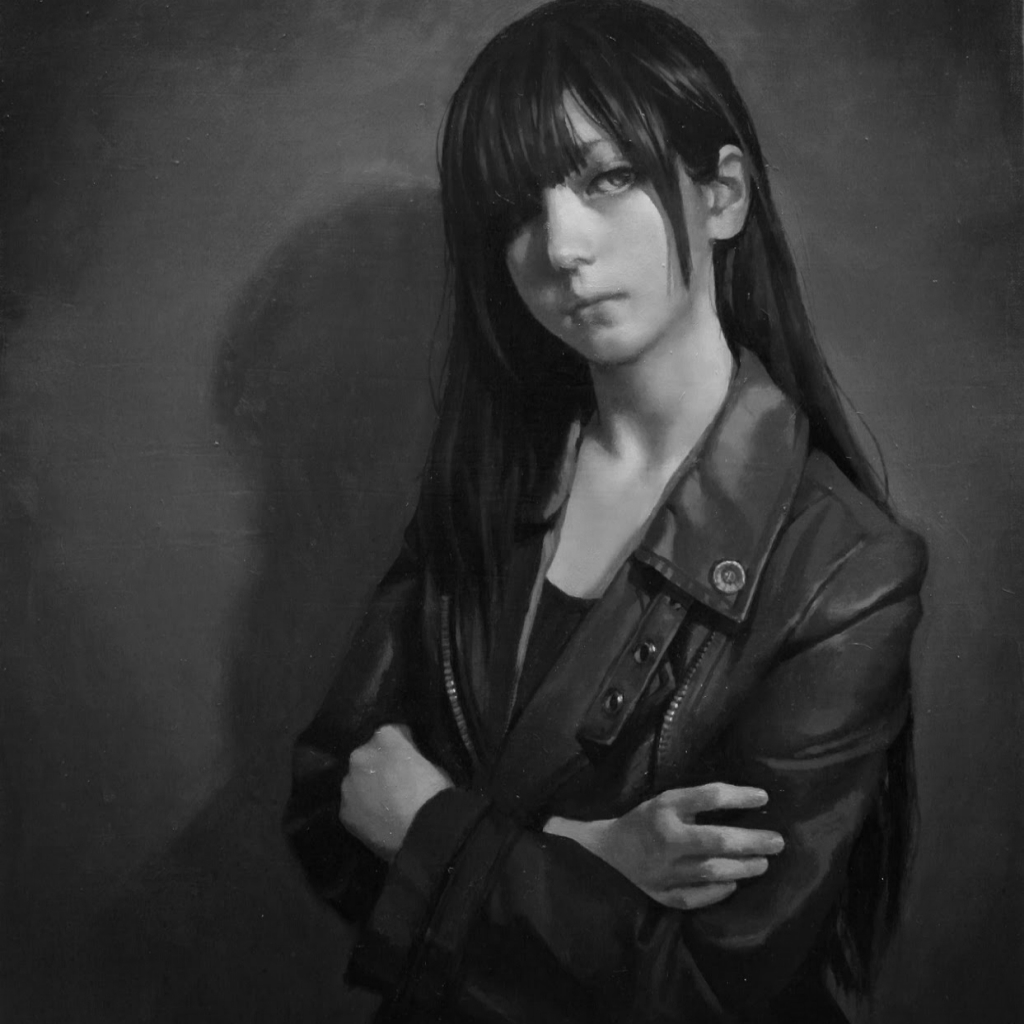
\includegraphics[width=.9\linewidth]{/home/loli/Documents/Workspace/Haskell/Class/531/eecs531-jxo136/Assignment2/data/lowHighPass/girl/army-grey.png}
\begin{itemize}
\item here is the original image
\end{itemize}
\item \texttt{computeAbsDiff "data/army.jpg" "girllow" lowPass 10}
\\

\includegraphics[width=.9\linewidth]{/home/loli/Documents/Workspace/Haskell/Class/531/eecs531-jxo136/Assignment2/data/lowHighPass/girl/low-10/girllow-10.png}
\begin{itemize}
\item so this is the low pass filter with n = 10
\item Notice how we keep the overall outline of the girl
\item overall not that great on this object
\end{itemize}
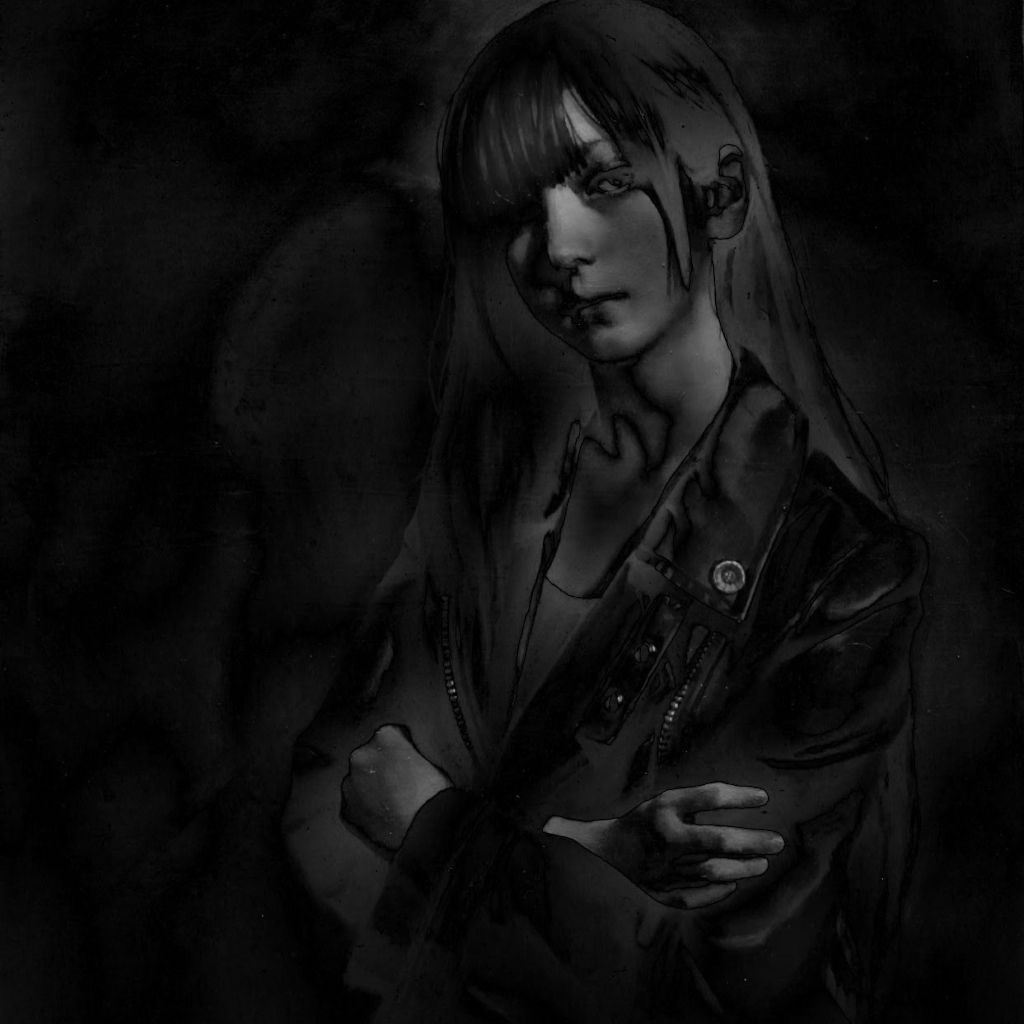
\includegraphics[width=.9\linewidth]{/home/loli/Documents/Workspace/Haskell/Class/531/eecs531-jxo136/Assignment2/data/lowHighPass/girl/low-10/abs-diff-girllow-10.png}
\begin{itemize}
\item here is the absolute difference between the original image and the
low pass filter
\item Notice all the detail that was left out of the lowPass
\end{itemize}
\item \texttt{computeAbsDiff "data/army.jpg" "girlhigh" highPass 10} \\
  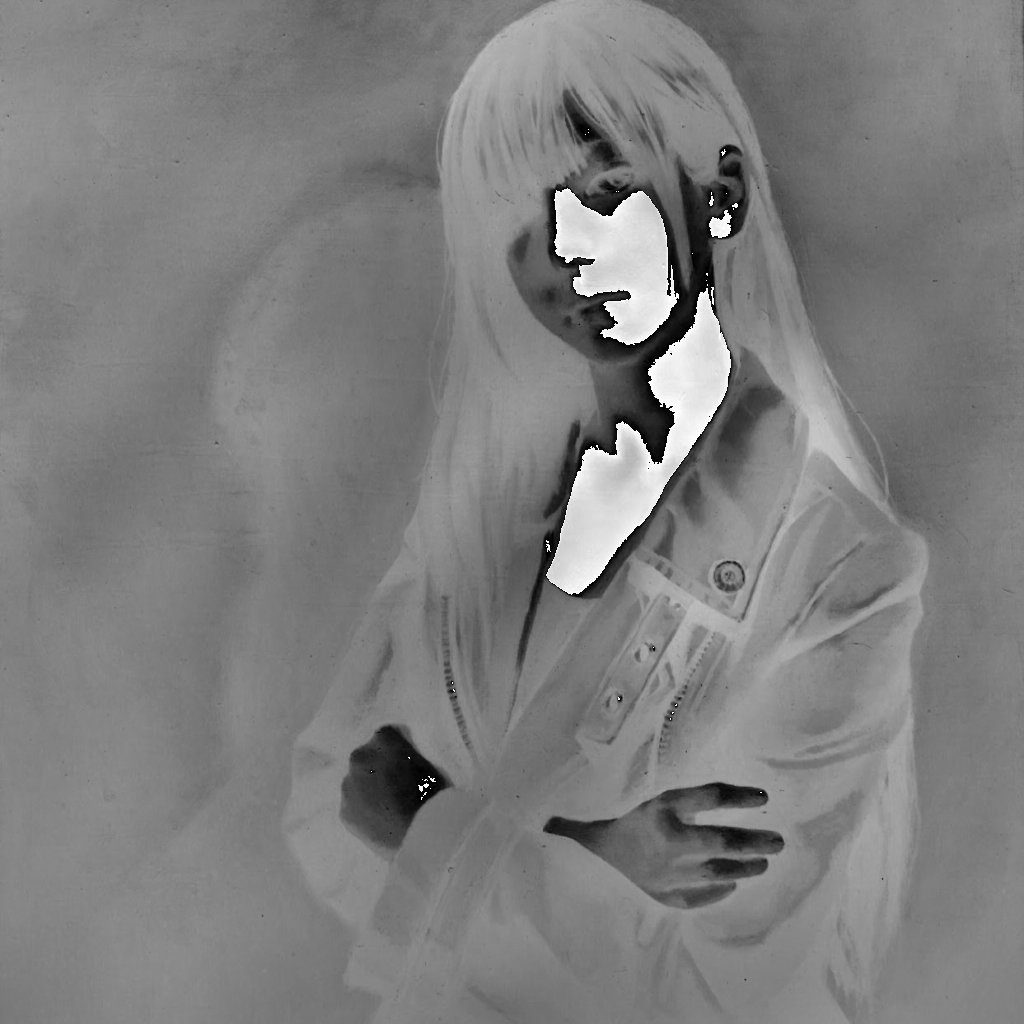
\includegraphics[width=.9\linewidth]{/home/loli/Documents/Workspace/Haskell/Class/531/eecs531-jxo136/Assignment2/data/lowHighPass/girl/high-10/girlhigh-10.png}
  \\
\begin{itemize}
\item here Ι run the high pass algorithm with zeroing out everything
passed 10
\item Quite a lot of the detail is captured
\end{itemize}

\includegraphics[width=.9\linewidth]{/home/loli/Documents/Workspace/Haskell/Class/531/eecs531-jxo136/Assignment2/data/lowHighPass/girl/high-10/abs-diff-girlhigh-10.png}
\begin{itemize}
\item This is the difference between the two images, and as can be seen,
the overall structure of her hair is formed in the difference
demonstrating that bit of information is missed
\end{itemize}
\end{itemize}
\item Bunny Image
\label{sec-1-3-2}
\begin{itemize}
\item Another image I did a lot of tests on was this bunny image, I will
post the results of high and low on 20 and 70 respectively. \\
  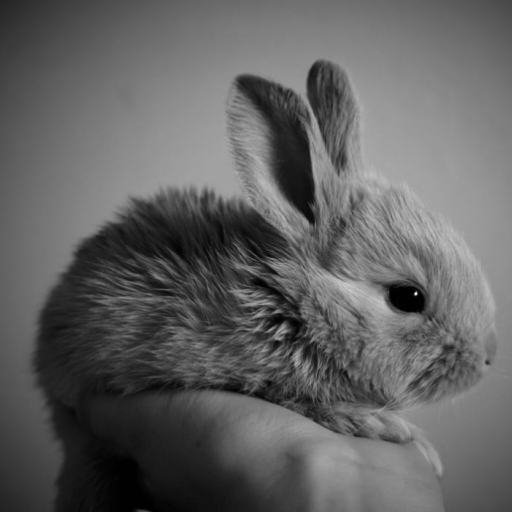
\includegraphics[width=.9\linewidth]{/home/loli/Documents/Workspace/Haskell/Class/531/eecs531-jxo136/Assignment2/data/lowHighPass/bunny/bunny-grey.png}
\begin{itemize}
\item here is the original image
\end{itemize}
\item \uline{70 tests}
\begin{itemize}
\item \texttt{computeAbsDiff "data/bunny.png" "bunnyhigh-70" highPass 70} \\
    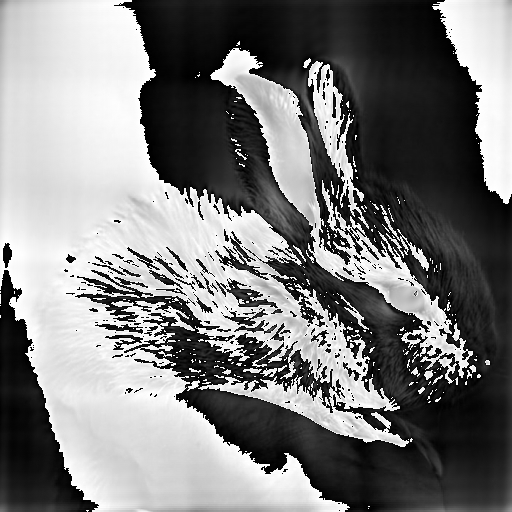
\includegraphics[width=.9\linewidth]{/home/loli/Documents/Workspace/Haskell/Class/531/eecs531-jxo136/Assignment2/data/lowHighPass/bunny/70/high/bunyhigh-70.png}
\begin{itemize}
\item Here we can see the high pass filter on the bunny, it keeps the
nice fine details but overall we lose the shape outside of the
sharp details.
\end{itemize}
\item 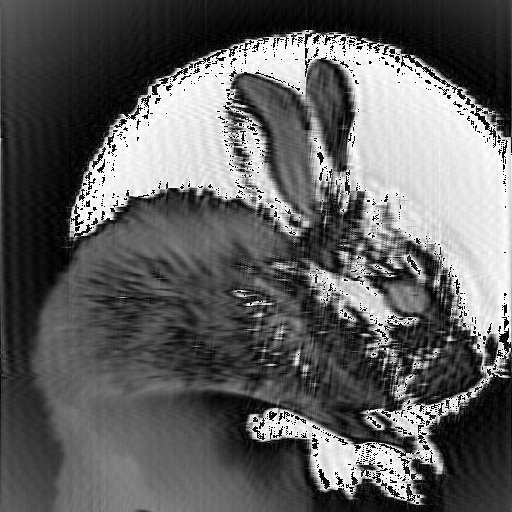
\includegraphics[width=.9\linewidth]{/home/loli/Documents/Workspace/Haskell/Class/531/eecs531-jxo136/Assignment2/data/lowHighPass/bunny/70/high/abs-diff-bunyhigh-70.png}
\begin{itemize}
\item The absolute difference confirms that pretty much most
information is lost
\end{itemize}
\item \texttt{computeAbsDiff "data/bunny.png" "bunnylow-70" highPass 70} \\
    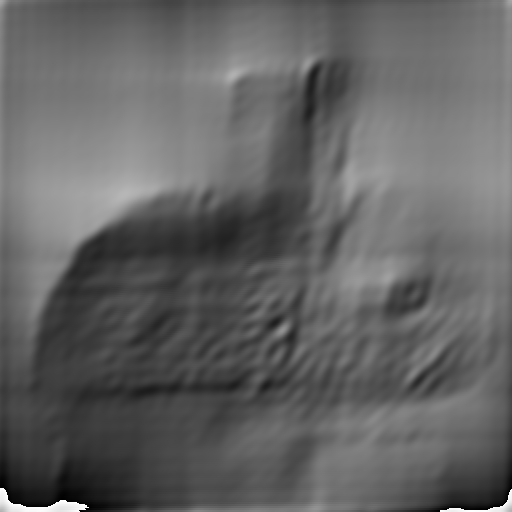
\includegraphics[width=.9\linewidth]{/home/loli/Documents/Workspace/Haskell/Class/531/eecs531-jxo136/Assignment2/data/lowHighPass/bunny/70/low/bunylow-70.png}
\begin{itemize}
\item This is the lowPass Filter on the bunny with 70
\item as we can see the overall shape of the bunny is kinda reserved,
but all fine detials are missing
\end{itemize}
\item 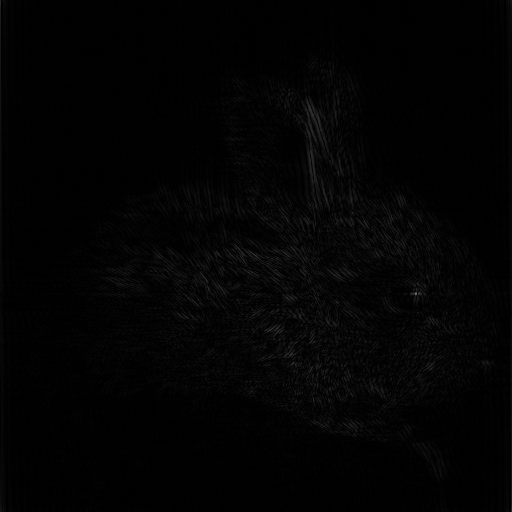
\includegraphics[width=.9\linewidth]{/home/loli/Documents/Workspace/Haskell/Class/531/eecs531-jxo136/Assignment2/data/lowHighPass/bunny/70/low/abs-diff-bunylow-70.png}
\begin{itemize}
\item The Absolute difference confirms this as, as the absolute
difference contains a lot of detail
\end{itemize}
\end{itemize}
\item \uline{20 tests}
\begin{itemize}
\item \texttt{computeAbsDiff "data/bunny.png" "bunnyhigh-20" highPass 20} \\
    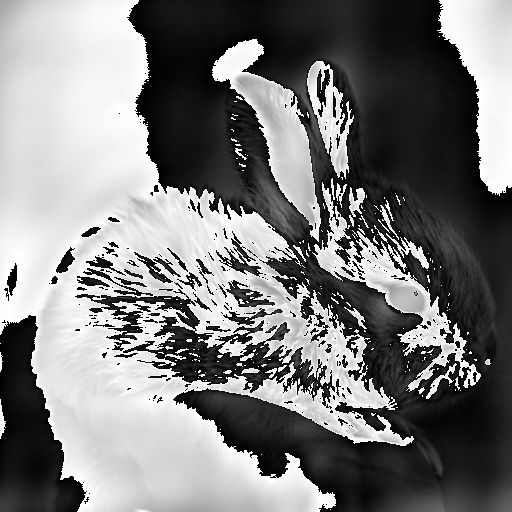
\includegraphics[width=.9\linewidth]{/home/loli/Documents/Workspace/Haskell/Class/531/eecs531-jxo136/Assignment2/data/lowHighPass/bunny/20/high/bunyhigh-20.png}
\begin{itemize}
\item this is the high pass filter on the bunny, but instead with a
size of 20, compared to 70 more details can be seen and the bunny
is starting to look a lot better outlined than with 20
\end{itemize}
\item 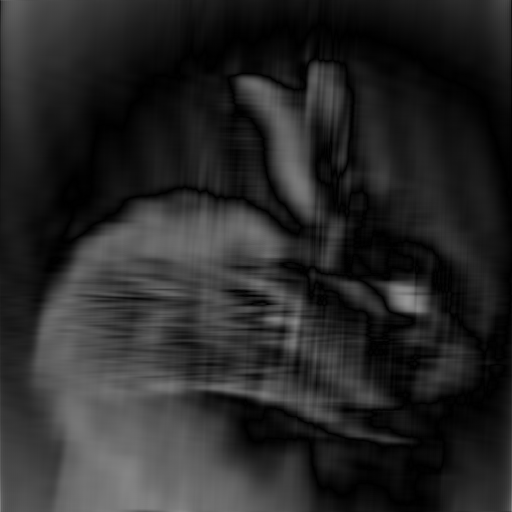
\includegraphics[width=.9\linewidth]{/home/loli/Documents/Workspace/Haskell/Class/531/eecs531-jxo136/Assignment2/data/lowHighPass/bunny/20/high/abs-diff-bunyhigh-20.png}
\begin{itemize}
\item This is the absolute difference, compared to the 70 this is a
lot more blurry and disjoint, with only parts of the general shape
being missing
\end{itemize}
\item \texttt{computeAbsDiff "data/bunny.png" "bunnylow-20" highPass 20} \\
    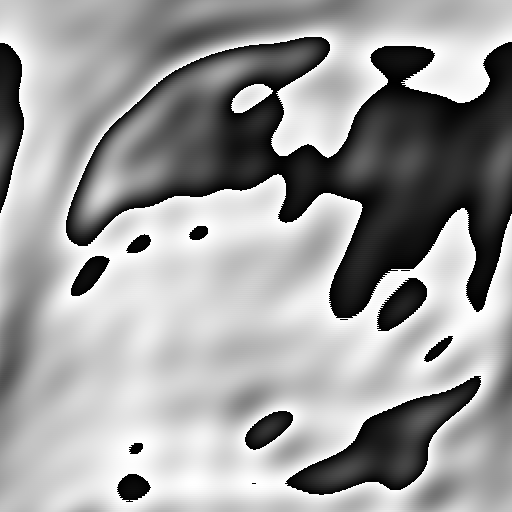
\includegraphics[width=.9\linewidth]{/home/loli/Documents/Workspace/Haskell/Class/531/eecs531-jxo136/Assignment2/data/lowHighPass/bunny/20/low/bunylow-20.png}
\begin{itemize}
\item This is the low pass filter with 20, compared to 70 pretty much
all detail is gone and only the general shape being intact
\end{itemize}
\item 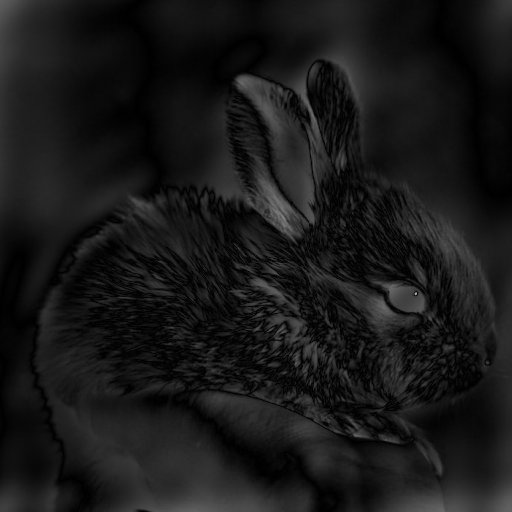
\includegraphics[width=.9\linewidth]{/home/loli/Documents/Workspace/Haskell/Class/531/eecs531-jxo136/Assignment2/data/lowHighPass/bunny/20/low/abs-diff-bunylow-20.png}
\begin{itemize}
\item This is the absolute difference, as can be noticed, the detail
of the bunny is much greater.
\end{itemize}
\end{itemize}
\end{itemize}
\end{enumerate}
\end{enumerate}
% Emacs 25.3.1 (Org mode 8.2.10)
\end{document}